
\documentclass{mproj}
\usepackage{graphicx}

\usepackage{url}
\usepackage{fancyvrb}
\usepackage[final]{pdfpages}
\usepackage{times}

%\usepackage[nottoc,numbib]{tocbibind}
\usepackage[nottoc]{tocbibind}

% for alternative page numbering use the following package
% and see documentation for commands
%\usepackage{fancyheadings}


% other potentially useful packages
%\uspackage{amssymb,amsmath}
%\usepackage{url}
%\usepackage{fancyvrb}
%\usepackage[final]{pdfpages}
\usepackage{CTEX}
\usepackage{comment}

\usepackage[section]{placeins} % 添加这个以限制浮动体跨越节的边界

\usepackage{listings}
\usepackage{xcolor}  % 用于定义颜色

\usepackage{amsmath}

\usepackage{hyperref}
\usepackage{cleveref}
\crefname{figure}{Figure}{Figures} % 设置 \cref 引用图像的格式

\begin{document}

%%%%%%%%%%%%%%%%%%%%%%%%%%%%%%%%%%%%%%%%%%%%%%%%%%%%%%%%%%%%%%%%%%%
%Towards Faster Parallelism: Performance-Driven Workstealing Scheduling in YewPar
\title{Towards Faster Combinatorial Search: Performance-Driven Workstealing Policy in YewPar}
\author{Hao Xie}
\date{24th August 2023}
\maketitle
%%%%%%%%%%%%%%%%%%%%%%%%%%%%%%%%%%%%%%%%%%%%%%%%%%%%%%%%%%%%%%%%%%%

%%%%%%%%%%%%%%%%%%%%%%%%%%%%%%%%%%%%%%%%%%%%%%%%%%%%%%%%%%%%%%%%%%%
\begin{abstract}
    abstract goes here
\end{abstract}
%%%%%%%%%%%%%%%%%%%%%%%%%%%%%%%%%%%%%%%%%%%%%%%%%%%%%%%%%%%%%%%%%%%

%%%%%%%%%%%%%%%%%%%%%%%%%%%%%%%%%%%%%%%%%%%%%%%%%%%%%%%%%%%%%%%%%%%
\educationalconsent

%%%%%%%%%%%%%%%%%%%%%%%%%%%%%%%%%%%%%%%%%%%%%%%%%%%%%%%%%%%%%%%%%%%

\newpage
%%%%%%%%%%%%%%%%%%%%%%%%%%%%%%%%%%%%%%%%%%%%%%%%%%%%%%%%%%%%%%%%%%%
\section*{Acknowledgements}

acknowledgements go here

%%%%%%%%%%%%%%%%%%%%%%%%%%%%%%%%%%%%%%%%%%%%%%%%%%%%%%%%%%%%%%%%%%%
\tableofcontents
%%%%%%%%%%%%%%%%%%%%%%%%%%%%%%%%%%%%%%%%%%%%%%%%%%%%%%%%%%%%%%%%%%%

%%%%%%%%%%%%%%%%%%%%%%%%%%%%%%%%%%%%%%%%%%%%%%%%%%%%%%%%%%%%%%%%%%%
\chapter{Introduction}\label{intro}

精确组合搜索对于包括约束编程、图匹配和计算代数在内的广泛应用都是必不可少的。
而组合问题是通过系统地探索搜索空间来解决的,这样做在理论上和实践中都很难计算,
其中精确搜索则是探索整个搜索空间并给出可证明的最佳答案。
概念上精确的组合搜索通过生成和遍历代表备选选项的(巨大的)树来进行。
结合并行性、按需树生成、搜索启发式和剪枝可以减少精确搜索的执行时间。
由于巨大且高度不规则的搜索树,并行化精确组合搜索是极具挑战性的.


而其中有名为YewPar\cite{10.1145/3332466.3374537}的框架,这是第一个用于精确组合搜索的可扩展并行框架。
YewPar旨在允许非专业用户从并行中受益;
重用编码为算法骨架的并行搜索模式(to reuse parallel search patterns encoded as algorithmic
skeletons);并能在多个并行架构上运行。

与此同时,随着并行计算和多核处理器的普及,有效的任务调度变得越来越重要.
能并行加速搜索是YewPar的一个关键特性,这是通过各个节点的多个worker在本地任务池无任务时向其它节点的任务池窃取任务来实现节点空闲资源的利用。
而YewPar在本地任务池无任务时,是随机选取节点来窃取任务的,
其中Workstealing是一种被广泛研究和应用的并行调度策略,
它允许空闲的处理器从繁忙的处理器中“窃取”任务。
然而,很多如YewPar这样的workstealing调度器往往采用偏随机窃取的策略,
这往往会导致不必要的开销和延迟,浪费了大量试探窃取任务的时间,同时导致各节点的相对负载不均衡,延长了最终完成的时间。
目前也有很多关于workstealing的改进,但是不能很好的兼顾到低开销,去中心化,高负载均衡,高性能,高可扩展性等特性.


相比之下,本文提出了Performance-Driven Workstealing Policy,
并为之设计了新的框架能定期监测与传输多项有价值的数据,
并计算缓存最优窃取目标节点,
它能够以低成本搜集多项性能指标,如各节点的任务执行时间、处理器的工作/空闲时间比例和任务池获取的耗时,
并通过自研的Time-Optimized Workstealing Strategy算法计算出最优窃取目标节点并缓存和定时刷新,
当有worker空闲时便能直接从缓存获取最近一段时间的最优窃取目标,从而能很好的在多节点去中心化的环境下以较低成本缩短完成全部任务所需的时间.


本文对具体的设计与实现细节进行了剖析,
其中Performance-Driven Workstealing Policy在搜集性能参数时采用了平台无关与去中心化的设计,
一方面并不涉及具体的系统参数调用命令,而是从YewPar内部和底层的HPX\cite{10.1145/2676870.2676883}框架进行数据收集,从而能够在不同的硬件平台上正常运行;
另一方面没有单一的节点负责收集所有节点的性能参数,而是各节点各自收集本地的性能参数,并通过HPX的分布式通信机制分享本地处理后的数据,
同时获取其它节点数据进行本地最优窃取目标计算,从而避免了单一节点的性能瓶颈.
其中Time-Optimized Workstealing Strategy的核心思想是计算各节点执行本地任务的所需时间的预期和获取节点任务池任务的耗时的预期,
并优先选取所需时间预期最大的节点同时尽量缩短不必要的获取任务的额外耗时,从而降低各节点的worker空闲率的同时缩短完成全部任务所需的时间.
其中定时刷新最优窃取目标缓存的任务由一种动态调整刷新时间的自动刷新任务来主要负责,各节点都会部署一个这样的刷新器,
它通过间隔一个动态时间后执行刷新性能参数信息并计算最优窃取目标最后将最优目标进行缓存来实现刷新最优窃取目标缓存的目的.
而空闲的worker则会在试图获取缓存目标任务失败时进行一次称为辅助刷新的操作,帮助此时可能处在休眠的刷新器进行刷新最优窃取目标缓存的任务.
这些工作结合起来便能够实现Performance-Driven Workstealing Policy的加速效果.


本文同时对改进workstealing策略后的YewPar进行了评估,
评估在具有多核机器的Beowulf集群上进行,
结果表明,改进后的YewPar在不同节点数量和线程下相比原YewPar平均能够获得更好的性能,
能在不影响搜索结果的情况下不同程度的有效缩短执行完全部任务所需的时间.


%%%%%%%%%%%%%%%%%%%%%%%%%%%%%%%%%%%%%%%%%%%%%%%%%%%%%%%%%%%%%%%%%%%
\chapter{Survey}\label{survey}

\section{组合搜索}
\begin{comment}
在计算机科学和人工智能中,组合搜索是一种用于在给定的搜索空间中找到解决方案的方法。
经典的组合搜索问题包括解决八皇后难题或评估具有大型游戏树的游戏中的动作,例如黑白棋或国际象棋。
这种搜索特别适用于那些解空间巨大并且不可能穷举所有解决方案的问题。
一些算法保证找到最优解,而另一些算法可能只返回在已探索的状态空间部分中找到的最佳解。
通过分支与限界技术或采用启发式方法,组合搜索能够有效地减少搜索空间,并更快地找到解决方案。
\end{comment}

\subsection{并行组合搜索(Parallel Combinatorial Search)与YewPar}
随着现代计算机硬件的发展,特别是多核处理器和分布式系统的普及,
利用并行性来加速组合搜索已经成为研究的热点.
并行组合搜索的目标是将搜索空间分解成多个部分,以便可以在多个处理单元上同时执行,从而加速解决方案的发现。

YewPar是一个专为组合搜索设计的并行框架.
它提供了一套强大的工具和策略,允许开发者轻松地并行化他们的搜索算法.
YewPar的主要特点是其灵活性和可扩展性,使其能够应对各种复杂的搜索场景.
其中,workstealing是YewPar中用于任务调度的核心策略,
它允许处理器在本地任务队列为空时从其他处理器窃取任务,确保所有处理器都能保持忙碌,从而提高整体性能。

\subsubsection{Performance Anomalies}
\label{sec:performance_anomalies}
搜索算法依赖于排序启发式方法尽早找到有用的节点,
例如决策问题中的目标节点,
或者分支限界优化问题中的一个强约束节点。为了利用这些启发式方法,
搜索按从左到右的顺序进行(在树的所有深度上).
因此,访问节点的顺序搜索具有关于搜索树的完整信息,例如
来自它左侧的所有节点的当前最佳解,并且搜索是确定性的。
并行搜索在没有完整的左侧信息的情况下推测性地搜索子树,
并可能从从右到左的信息流中受益。但是,这种推测意味着
并行搜索可能比相同的顺序搜索执行更多的工作。
因此,并行搜索因性能异常而臭名昭著\cite{10.1007/3-540-60321-2_29}.
有害的异常是当w个工作线程上的运行时间超过w-1个工作线程时发生的。
在这里,额外的工作可能超过额外计算资源的好处,
或者额外的计算资源可能会破坏搜索启发式方法。
加速异常是超线性的加速,通常是由于从右到左的知识流动,
通过允许比顺序搜索中更多的修剪来减少总体工作量。
异常的存在使得推理搜索应用的并行性能变得困难。
Yew-Par旨在避免有害的异常,同时允许加速异常;
\cite{ARCHIBALD201892}报告了一个专门的搜索框架,该框架仔细控制异常以提供可复制的性能保证。

\section{workstealing}
Workstealing 是并行编程中的一个核心概念。
其主要优点在于分散调度,让每个处理器自主地管理其任务队列,从而显著降低了全局同步所带来的开销.
众多并行框架和库,如 Cilk、TBB 和 OpenMP,都已经采纳了这种方法。

在workstealing策略中,系统内的每个处理器都有自己的待执行任务队列.
每个任务都由一系列指令组成,这些指令需要按顺序执行。
但在执行的过程中,一个任务还可能生成新的子任务.
这些子任务被初步放入生成它们的任务所在的处理器队列.
当某处理器的任务队列为空时,它会尝试从其他处理器的队列中“窃取”任务.
这样,workstealing 实际上将任务调度到了空闲的处理器上,
并保证了只有在所有处理器都繁忙时才会发生调度开销.\cite{10.1145/1248377.1248396}

与workstealing形成对比的是工作共享策略,
它是动态多线程调度的另一种方法。
在工作共享中,新产生的任务会被立即调度到一个处理器上执行。
相较于此,workstealing减少了处理器间的任务迁移,
因为当所有处理器都繁忙时,这种迁移是不会发生的.\cite{10.1145/324133.324234}

尽管如此,传统的随机窃取策略在多节点复杂环境中往往有较大的开销.
这些开销主要来源于“窃贼”在集群中随机地探测节点以寻找“受害者”.
加之集群规模的不均匀分布,这种问题变得更为严重,
导致系统消息量过大以及“窃贼”由于多次窃取失败和网络延迟而产生的长时间饥饿状态.
尽管关于workstealing的优化尝试从未停歇,
例如通过建立固定的通道来匹配任务饥饿和任务丰富的节点\cite{10.1145/2851141.2851175},
但至今仍未有一种通用的去中心化、低开销、跨平台且高效的策略出现。
workstealing仍处于针对各种应用环境进行持续优化的阶段。

\section{为什么要在YewPar中设计并使用新的workstealing策略}

虽然YewPar已经采用workstealing作为其核心的调度策略,
但随机发现一个有任务的节点并一直窃取其任务的方法可能导致不必要的开销和计算资源的空闲,
尤其是在不均匀的任务分布和各节点具有不均衡的计算资源下.
考虑到组合搜索的特性,任务之间可能存在巨大的执行时间差异,这使得随机窃取策略可能并不是最优选择。

为了更好地利用每个处理器的计算能力并减少不必要的通信开销,
YewPar需要一种更加智能的workstealing策略。
基于各节点性能的新的Performance-Driven Workstealing Policy正是为了解决这一问题而提出的。
通过低成本评估每个节点的性能如平均任务执行时间等,新策略可以更精确地刷新最优窃取目标,从而提高整体性能。

%%%%%%%%%%%%%%%%%%%%%%%%%%%%%%%%%%%%%%%%%%%%%%%%%%%%%%%%%%%%%%%%%%%
\chapter{Design and implementation}

\section{总体设计}

本文为了Performance-Driven Workstealing Policy设计了一套新的框架,
框架包含Scheduler Channel(主要负责监测与统计与传输节点所有workers的负载状态),
Performance Monitor(主要负责统计各项性能数据与发送各项处理后的本地性能数据,并计算和缓存最优窃取目标节点的id),
和Performance Policy(在本地任务池无任务时,主要负责从Performance Monitor获取最优窃取目标).

组件之间的关系大致如\cref{fig:overall_architecture}所示.
\begin{figure}[h] % 'h'表示图片尽量在当前位置
    \centering % 让图片居中显示
    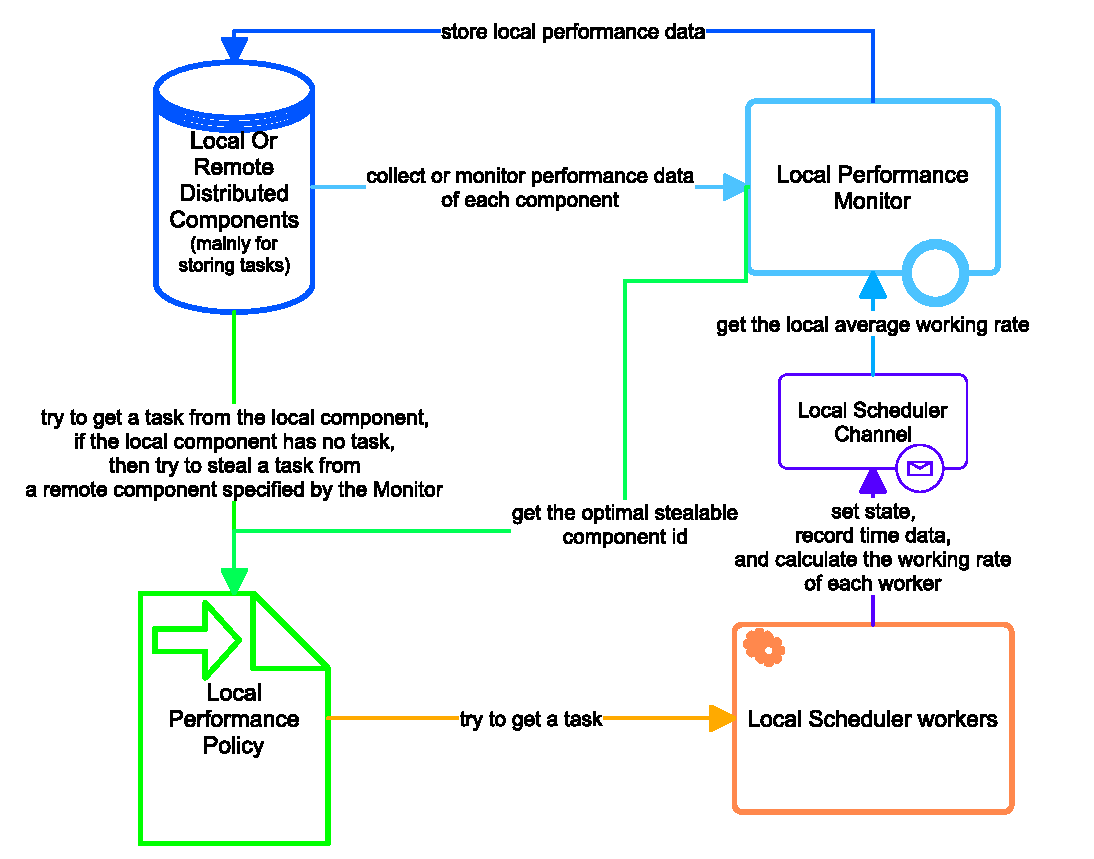
\includegraphics[width=0.9\textwidth]{images/overall_architecture.pdf} % 插入图片,设置图片宽度为文本宽度的80%
    \caption{Performance-Driven Workstealing Policy Architecture} % 提供图片的注解
    \label{fig:overall_architecture} % 为图片提供一个标签,以便在文档的其他地方引用
\end{figure}
\FloatBarrier

其中Performance Monitor主要负责各项性能数据的统计和传输,并计算和缓存最优窃取目标节点的id;
distributed component负责存储可供远程和本地访问的任务池和性能等数据,
通过hpx框架的action提供访问与改写操作;
Scheduler Channel提供接口让workers能更新自己当前负载状态并计算自己的负载数据,
workers负责从Performance Policy获取可执行的任务;
Performance Policy负责调取本地任务池任务或者从Performance Monitor获取最优窃取目标节点后窃取其任务池任务.

%%%%%%%%%%%%%%%%%%%%%%%%%%%%%%%%%%%%%%%%%%%%%%%%%%%%%%%%%%%%%%%%%%%

\section{性能数据收集与传输}
数据收集包含三部分:各节点负载情况,各节点剩余任务量,各节点获取任务池任务的耗时.
这三个参数将会为后续的最优窃取目标计算提供有力的数据支持.
同时,为了保障能以较低成本收集到更有效的数据,本文对三部分都进行了仔细的设计与优化.

\subsection{节点所有worker的负载情况}
首先,YewPar的System Stack大致如
\cref{fig:yewpar_system_stack}
\cite{10.1007/978-3-030-29400-7_14}
所示.

\begin{figure}[h] % 'h'表示图片尽量在当前位置
    \centering % 让图片居中显示
    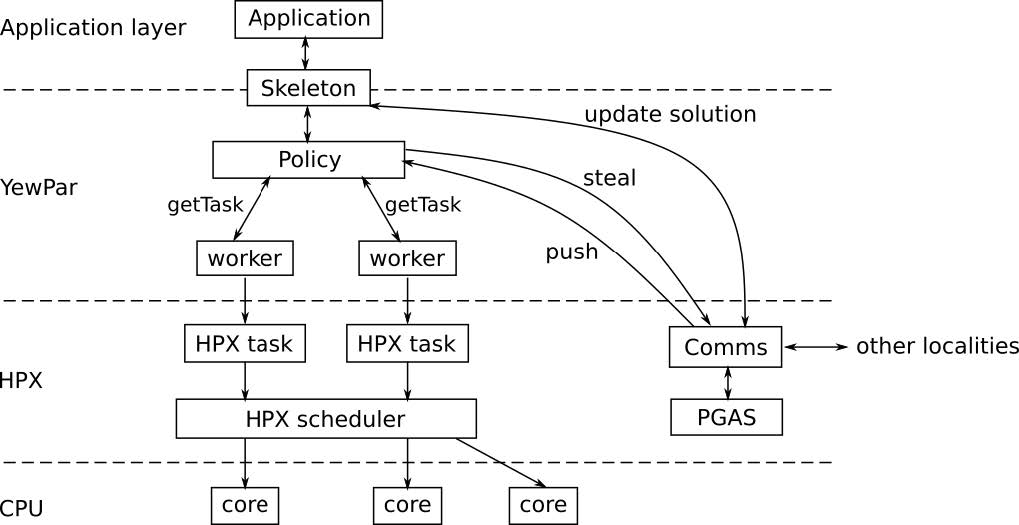
\includegraphics[width=0.9\textwidth]{images/YewPar_System_Stack.jpg} % 插入图片,设置图片宽度为文本宽度的80%
    \caption{YewPar System Stack} % 提供图片的注解
    \label{fig:yewpar_system_stack} % 为图片提供一个标签,以便在文档的其他地方引用
\end{figure}
\FloatBarrier

其中Policy负责被worker调用时,通过自己的策略试图获取任务
(最终会从本地池获取或从其它节点任务池偷取任务),
真正负责执行任务的是YewPar的worker,
所以如果想要不依赖系统底层函数获得各节点的负载情况,就需要获取各节点的worker的负载情况.
本文对worker的工作流程进行了分析,如\cref{fig:period_of_worker}

\begin{figure}[h]
    \centering % 让图片居中显示
    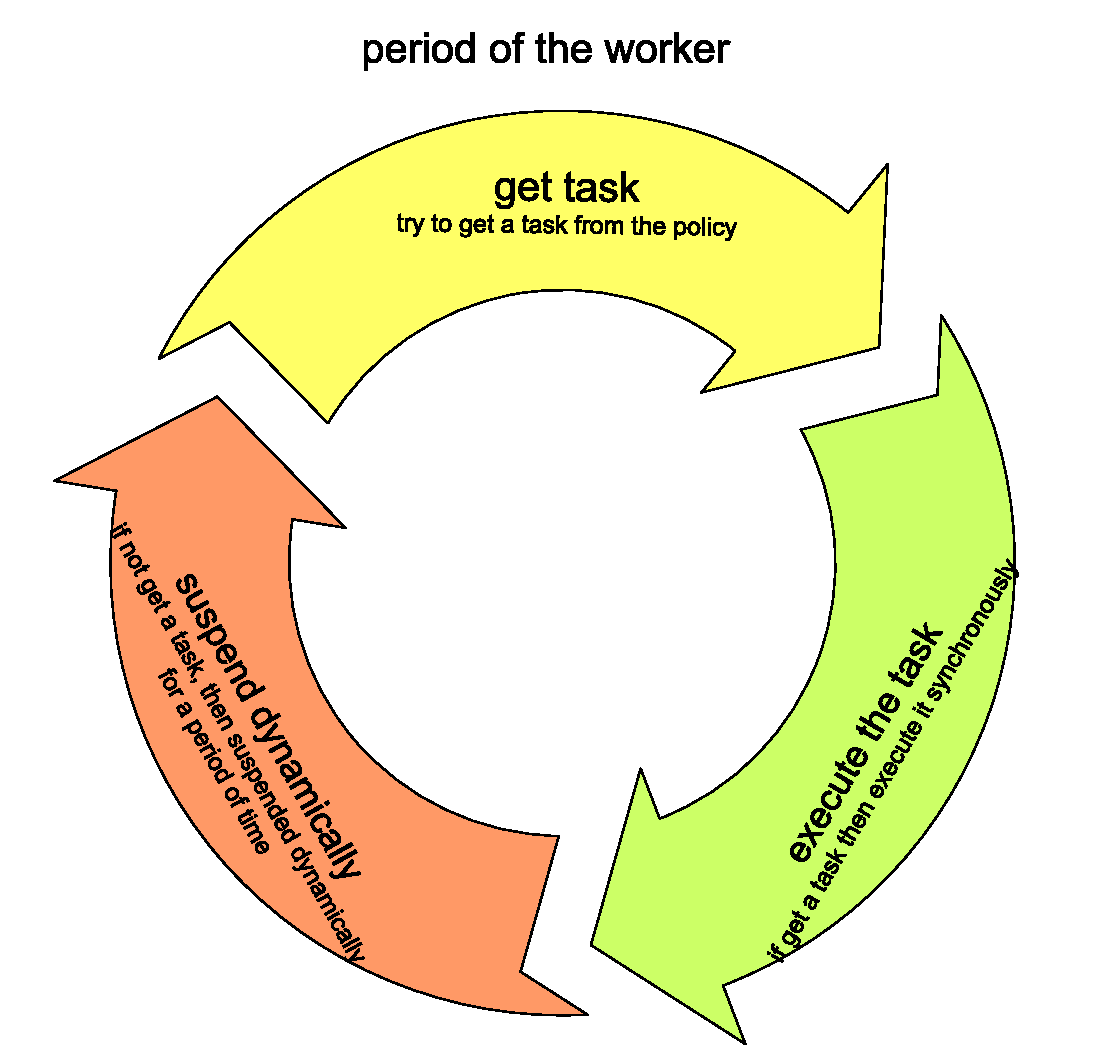
\includegraphics[width=0.7\textwidth]{images/period_of_worker.pdf} % 插入图片,设置图片宽度为文本宽度的80%
    \caption{period of the worker} % 提供图片的注解
    \label{fig:period_of_worker} % 为图片提供一个标签,以便在文档的其他地方引用
\end{figure}
\FloatBarrier

可以看出每个worker从创建到销毁之间,
它的生命周期都处在一个循环中,其中包含了三个可能的阶段:

1.调用Policy的getWork函数获取任务;

2.如果获取到任务则执行该任务;

3.如果没有获取到任务则休眠一段时间,
这段时间随着没有获取到任务的次数的增加而增加,当再次获取到任务时则时间重置

这三个阶段中,第一阶段是每次循环都会经历的阶段,
而第二阶段和第三阶段则是互斥关系,每次循环只会经历其中一个阶段.

如果需要分析worker的真实负载情况,
就需要以第二阶段为核心进行统计,
因为第二个阶段是worker真正执行任务的阶段,
它所消耗的时间是worker执行任务的时间,也就是有效的负载时间,
而其它阶段所消耗的时间则可以归类为worker的空闲时间,
因为这段时间并没有执行任何任务,也就是无效的负载时间.

由于原先一个周期未必能经历第二阶段,
所以为了避免更新无效数据,
本文对worker的生命周期判定进行了重定义,
以一个任务的执行完毕为一个新周期的开始,
以一个任务的开始为一个周期的结束,
这样便能保证每个周期都能经历第二阶段,也就是执行任务的阶段.

在此理论基础上,本文设计了如\cref{fig:worker_collect_calculate}的一套完整的数据收集方案,

\begin{figure}[h]
    \centering % 让图片居中显示
    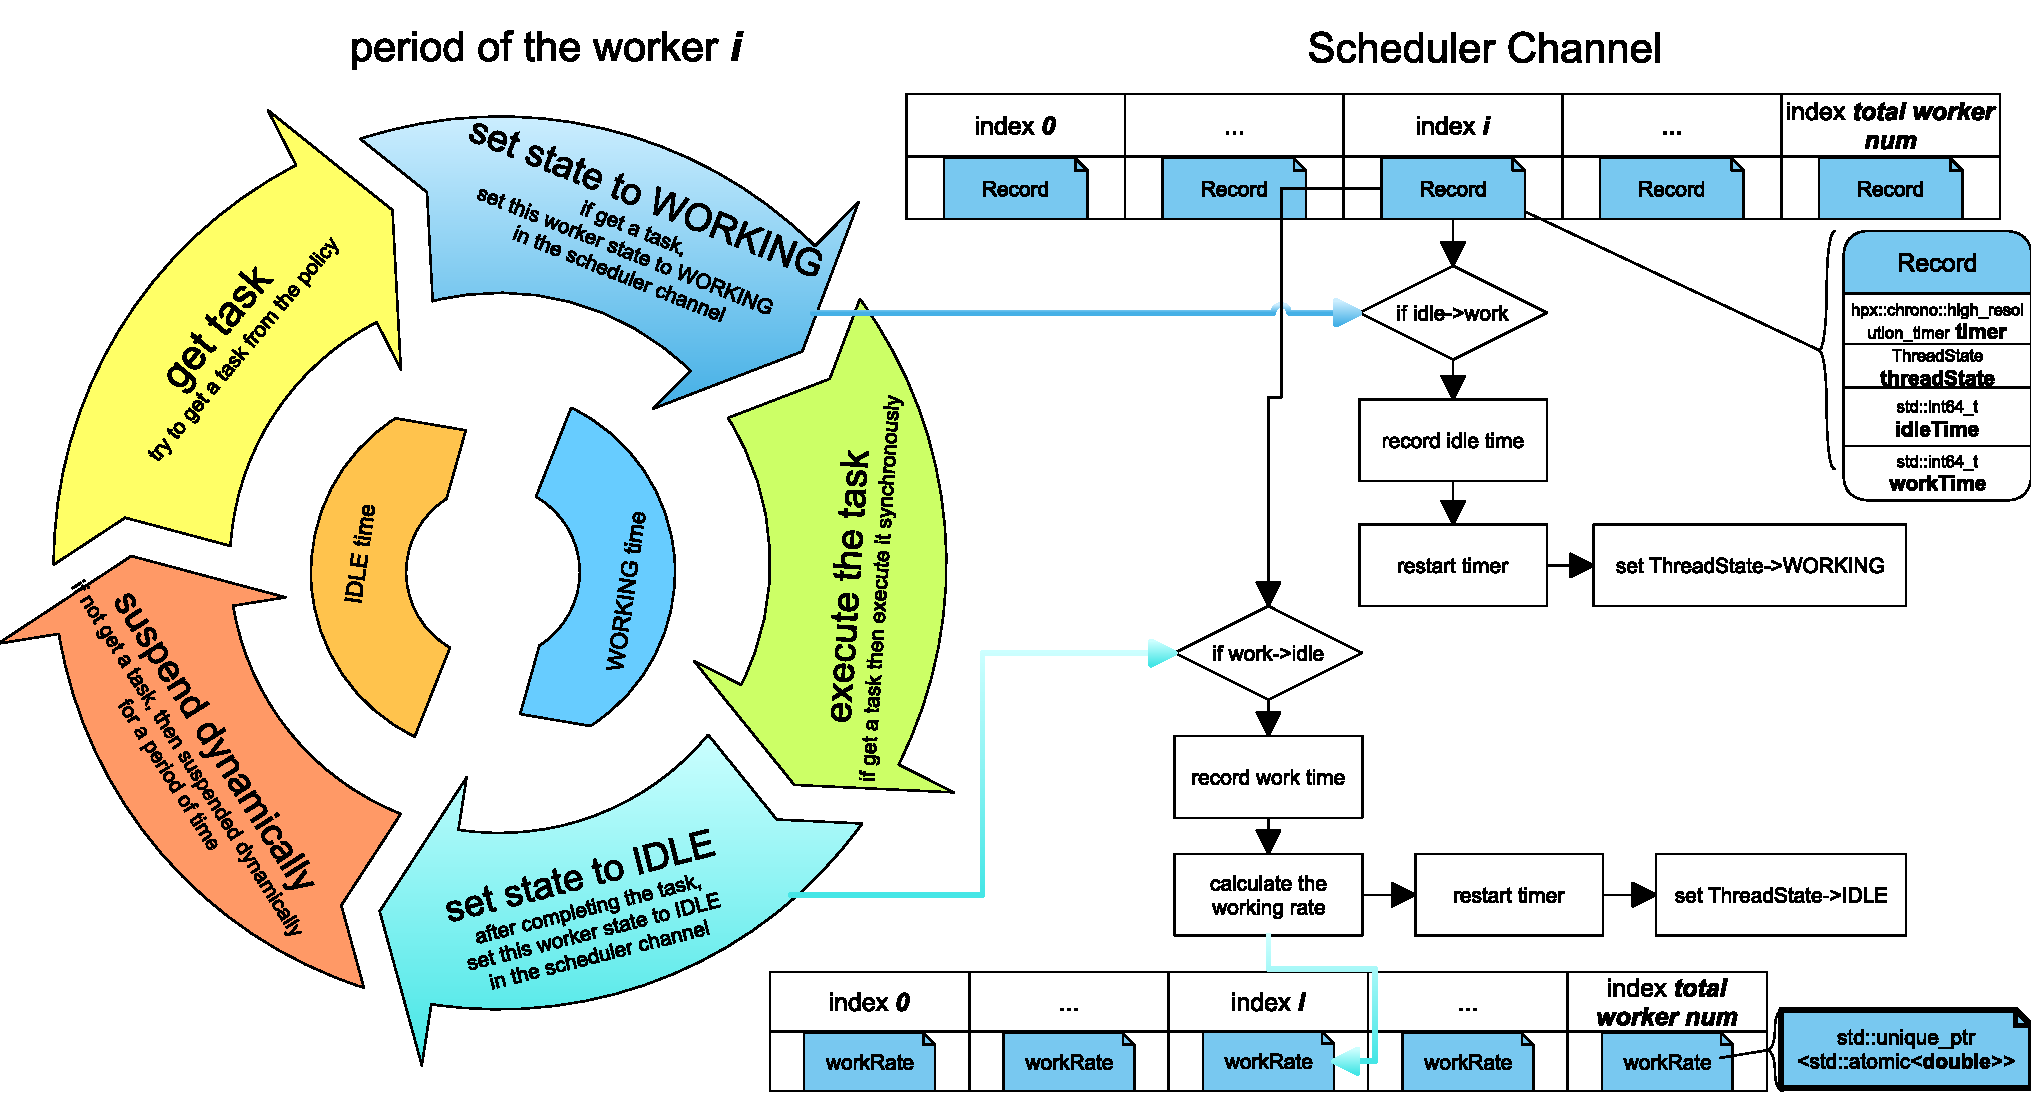
\includegraphics[width=1.0\textwidth]{images/worker_collect_calculate.pdf} % 插入图片,设置图片宽度为文本宽度的80%
    \caption{collect worker state to calculate the work load} % 提供图片的注解
    \label{fig:worker_collect_calculate} % 为图片提供一个标签,以便在文档的其他地方引用
\end{figure}
\FloatBarrier

通过在任务开始执行之前和执行完成后的位置插入探针代码,
让worker在执行任务前和完成任务后都去Scheduler Channel(一个辅助传输状态的channel)中更新自己的状态,
并计算自己的负载数据,
方便后续Performance-Driven Policy获取这些数据进行计算.

其中Scheduler Channel的统计数据主要由两组长度为workers数量的数组组成,
一组存储着特定的Record数据结构,
由一个计时器timer,一个当前状态threadState,一个当前周期的空闲时间idleTime和一个当前周期的工作时间workTime组成,
方便workers记录自己的具体各状态持续时间等数据,
由于设计采用一个record对应一个worker的方式,所以record可以不采用锁机制以提升性能;
另一组存储着采用特定算法计算得出的worker负载率数据workRate,
由被unique\_ptr包装的原子double类型组成,
由于可能有worker和Moninter同时访问,所以需要采用原子类型以保证在无锁机制下数据的正确性.

在"set state to WORKING"阶段,worker主要在channel更新自己这轮周期的空闲时间,并更改状态为WORKING;
而在"set state to IDLE"阶段,worker主要在channel更新自己这轮周期的工作时间,
并根据空闲与工作时间与历史workRate数据计算出当前的workRate,并更改状态为IDLE.

而计算最新的workRate的算法如\cref{eq:workrate}所示:

\begin{align}
    \text{workRate} & = \left( \ln\left( 2.72 + \frac{\text{workTime}}{\text{workTime} + \text{idleTime}} \right) \right. \notag   \\
                    & \qquad \times \left. \ln\left( 2.72 + (\text{workTime} + \text{idleTime}) \right) \times 0.65 \right) \notag \\
                    & \qquad + \text{workRate} \times 0.35 \label{eq:workrate}
\end{align}

公式目的是为了计算当前worker是否繁忙和计算速度是否较慢,主要分为三部分:
\begin{enumerate}
    \item $\ln\left( 2.72 + \frac{\text{workTime}}{\text{workTime} + \text{idleTime}} \right)$,
          是由于在每个周期中,如果WORKING状态的持续时间相对IDLE状态的持续时间比值越大,
          则说明当前任务量较大或者任务较为复杂,所以需要更多的时间来执行任务.
          同时为了避免数据过于敏感,所以采用了对数函数来降低数据的敏感度,
          使用了$(2.72+...)$是为了保证结果永远为正数.

    \item $\ln\left( 2.72 + (\text{workTime} + \text{idleTime}) \right)$,
          是因为如果当前周期的总持续时间越长,则说明当前任务较为复杂或者worker的性能较低,
          所以需要更多的时间来执行任务.
          同时也采用了对数函数来降低数据的敏感度.

    \item $(... \times 0.65 +\text{workRate} \times 0.35)$,
          这是采用了一种称为指数平滑\cite{GARDNER2006637}的算法,通过给与历史数据影响程度一定的系数,
          防止短期的波动给结果带来较大的影响,从而使得数据更加平滑和更具参考价值.
          而0.65和0.35则是经过多次测试后得出的一个较为合理的系数,
          既保留了一些历史参考,也较好地体现了最近的数据变化.
\end{enumerate}

最终,计算出的各个worker的workRate数据会通过提供的本地接口在计算总和并除以worker的数量后递交给Performance Monitor,
Performance Monitor会将本地workRate数据提交给local distributed component以供其它节点查询.


\subsection{各节点剩余任务量与获取花费时间收集}

性能数据还需要对各节点剩余任务量和获取花费时间进行收集,
具体实现如\cref{fig:tasks_detection}所示.

\begin{figure}[h]
    \centering % 让图片居中显示
    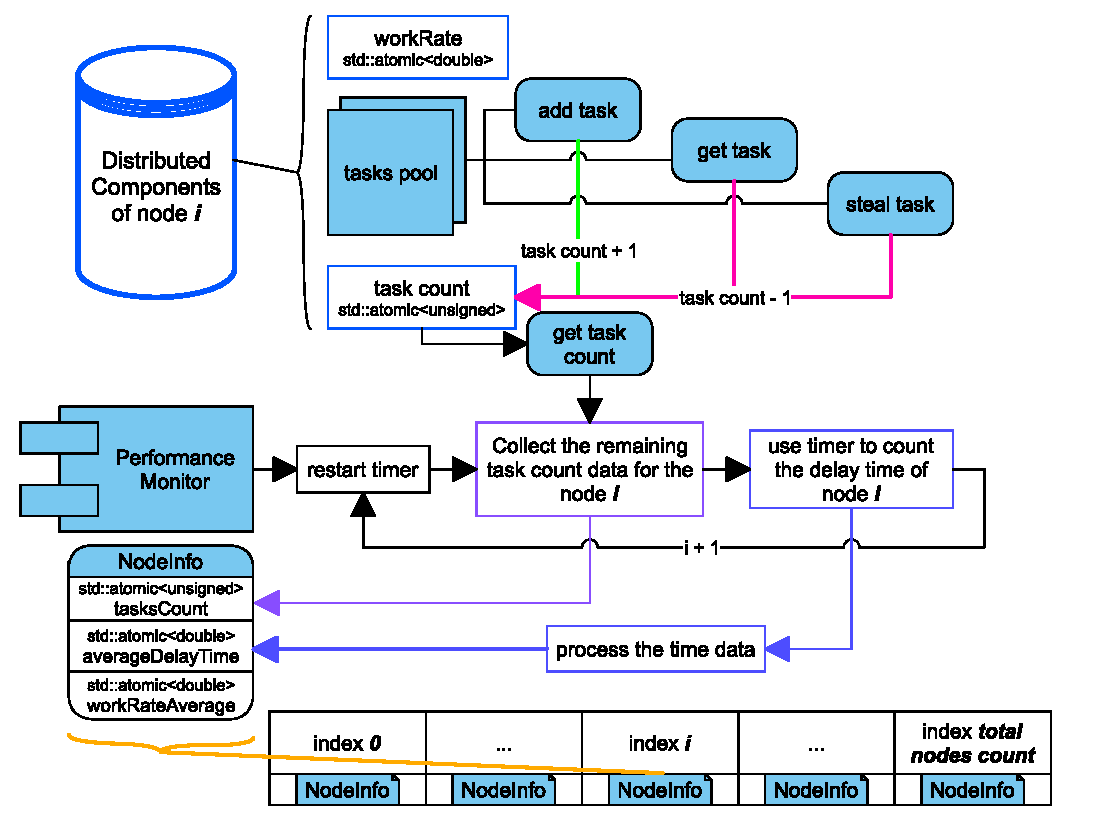
\includegraphics[width=0.98\textwidth]{images/tasks_detection.pdf} % 插入图片,设置图片宽度为文本宽度的80%
    \caption{collect tasks count and delay time} % 提供图片的注解
    \label{fig:tasks_detection} % 为图片提供一个标签,以便在文档的其他地方引用
\end{figure}
\FloatBarrier

在hpx分布式组件中包含了任务池与剩余任务数量,
任务池有三种分布式操作包含添加任务,获取任务与窃取任务,
所以在调用这三种操作时会进行检测并对剩余任务数进行更新.

而在Performance Monitor中,
会定时遍历并调用各节点的distributed component的接口获取节点的剩余任务数.
同时在获取时通过计时器计算获取节点任务数的耗时,并加以处理后进行存储,
存储会存储在一个长度为节点总数的数组的对应节点编号的位置的一个称为NodeInfo的数据结构中,
也采用了无锁的原子数据以低成本保证线程安全.

这里耗时反应了节点线程池的繁忙程度和节点之间的通讯延迟时间,
因为一方面任务数量是采用原子类型,在有数据修改时都会将其它修改或者读取请求延后,
那么当任务池繁忙时,往往会导致获取任务数的耗时增加;
另一方面由于各节点之间的通讯是通过hpx的分布式通讯机制进行的,
当进行"get task count"分布式操作时,中间的耗时也必然反应了节点间的通讯延迟情况.
后续通过这两项数据也会对最优窃取目标的计算有重要影响.

由于获取任务数耗时是一项时间数据,可能具有较大的数值与波动,所以需要处理后再存储,
处理公式为
\begin{align}
    \text{averageDelayTime}_i & = \ln\left(2.72 + \text{delayTime} \times \text{worker\_count}\right) \times 0.65 \notag               \\
                              & + \text{nodeInfoVector}[i]\texttt{->}\text{averageDelayTime} \times 0.35   \label{eq:averageDelayTime}
\end{align}
其中$i$为节点编号,$\text{delayTime}$为获取任务数的耗时,$\text{worker\_count}$为节点worker数量,
公式首先通过将延迟时间乘以本地的worker数量来反应综合节点的通讯耗时,
再同时参考\cref{eq:workrate}也通过对数函数与指数平滑来降低数据的敏感度,并使数据更加平滑和更具参考价值

\section{最优窃取目标计算与缓存}

在Performance Monitor通过性能收集机制获得了包括
各节点负载情况,各节点剩余任务量,各节点获取任务池任务的耗时等性能数据后,
Performance Monitor会通过各节点的数据计算出最优窃取目标节点,
并将其缓存起来以供后续Performance Policy获取.
其实现如\cref{fig:refresh_target}所示.

\begin{figure}[h]
    \centering % 让图片居中显示
    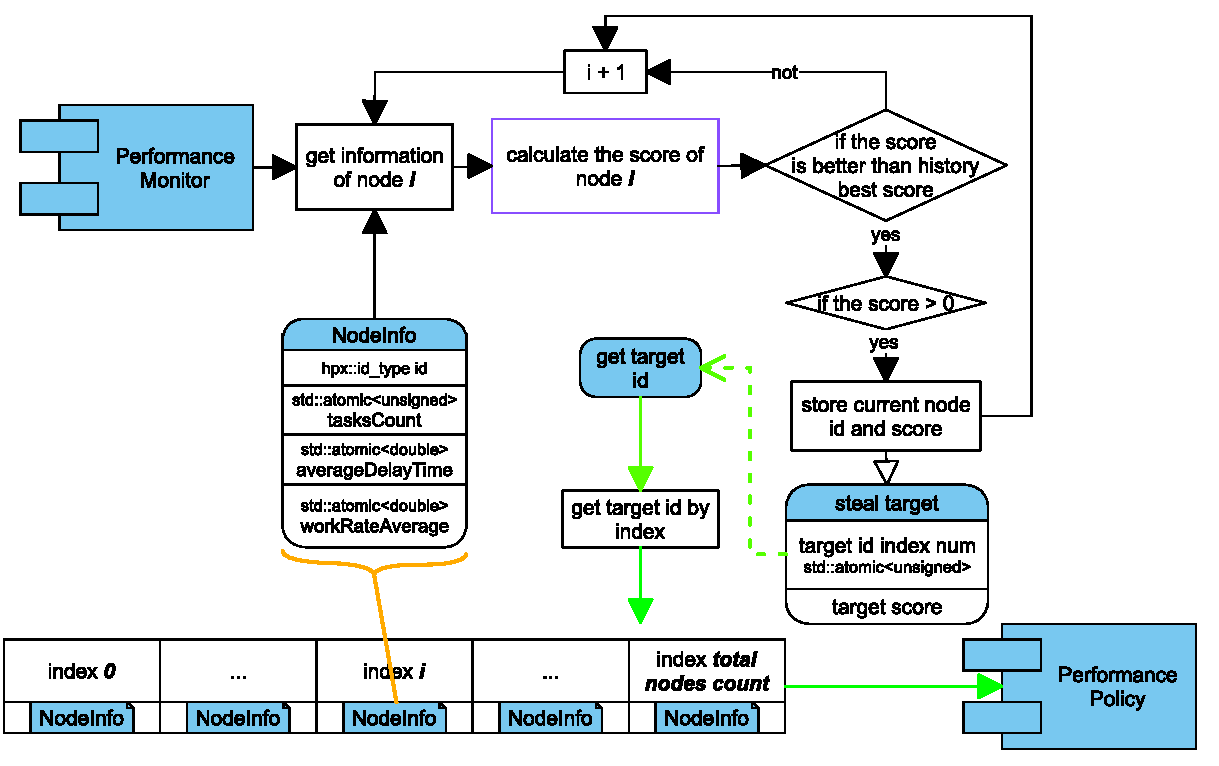
\includegraphics[width=1\textwidth]{images/refresh_target.pdf} % 插入图片,设置图片宽度为文本宽度的80%
    \caption{refresh the optimal steal target} % 提供图片的注解
    \label{fig:refresh_target} % 为图片提供一个标签,以便在文档的其他地方引用
\end{figure}
\FloatBarrier

这里整体流程也采用了无锁化的设计,通过的互相独立的节点结构和原子数据以低时间成本保证线程安全.

其中首先通过遍历各节点的NodeInfo数据结构中性能数据,来计算各节点的steal-worthiness score,
得分越高则说明越值得窃取,
其计算公式为
\begin{align}
    \text{score}_i & = \max\left(\text{nodeInfoVector}[i]\texttt{->}\text{workRateAverage}, 0.0001 \right) \notag \\
                   & \quad\times \text{nodeInfoVector}[i]\texttt{->}\text{tasksCount} \notag                      \\
                   & \quad - \text{nodeInfoVector}[i]\texttt{->}\text{averageDelayTime} \label{eq:score}
\end{align}

公式的核心思想是尽量减少预计耗时最长的节点的任务池任务数的同时一定程度减少浪费在窃取其任务上的时间,
所以先通过$\max\left(\text{nodeInfoVector}[i]\texttt{->}\text{workRateAverage}, 0.0001 \right)$
来避免过小的无意义数据对计算的干扰,
之后通过$\times \text{nodeInfoVector}[i]\texttt{->}\text{tasksCount}$来预估该节点执行完任务的大致剩余时间,
最后通过$- \text{nodeInfoVector}[i]\texttt{->}\text{averageDelayTime}$
来减去一定的获取任务预估的损耗时间.
最终得到的结果越大则一定程度上说明该节点越值得窃取.

在遍历完所有节点后,一般会得到一个最优的节点目标编号索引,
会将这个最优的节点目标编号索引数进行缓存,
当Performance Policy需要获取最优窃取目标的$id\_type$时,
会通过提供的查询接口,
通过索引再去节点数组里获取最优窃取目标节点的$id\_type$,
这样同时也保障了在hpx的$id\_type$类型无原子操作的情况下仍能保持无锁机制.

在判断最优窃取目标时,我们也需要判断窃取的成本是否高过了收益,
而这种情况往往发生在窃取过程的消耗时间大于了帮助目标节点完成任务所节省的时间,
这种情况下score往往会小于或者等于0,
所以设置了额外的判断条件,在score小于或者等于0的情况下不会缓存最优窃取目标.


\section{Refresh data and provide tasks mechanism}

在建立了一套从数据收集到计算最优窃取目标和缓存最优窃取目标的机制后,
我们还需要的问题,就是以何种频率去刷新各项数据.
虽然每一次刷新数据的开销都是相对很小的,
但是YewPar的worker数量会尽量占满本地的计算资源,
那么当worker繁忙时,过于频繁的刷新会导致worker的计算资源被占用,
从而一定程度影响YewPar的性能.
但是如果刷新的频率过低,则会导致数据的可靠性降低,
因为数据的实时性降低,
提供给其它节点的数据和缓存的其它节点数据都将不够准确,
甚至可能导致窃取到其它任务饥饿的节点,加剧不均衡的情况.

为解决这一问题,本文设计了一种双向动态刷新的刷新机制,
它由两种刷新方式组成,
一种是自动动态刷新任务方式,另一种是通过Performance Policy进行辅助刷新方式.
大致流程如\cref{fig:refresh_provide}所示.

\begin{figure}[h]
    \centering % 让图片居中显示
    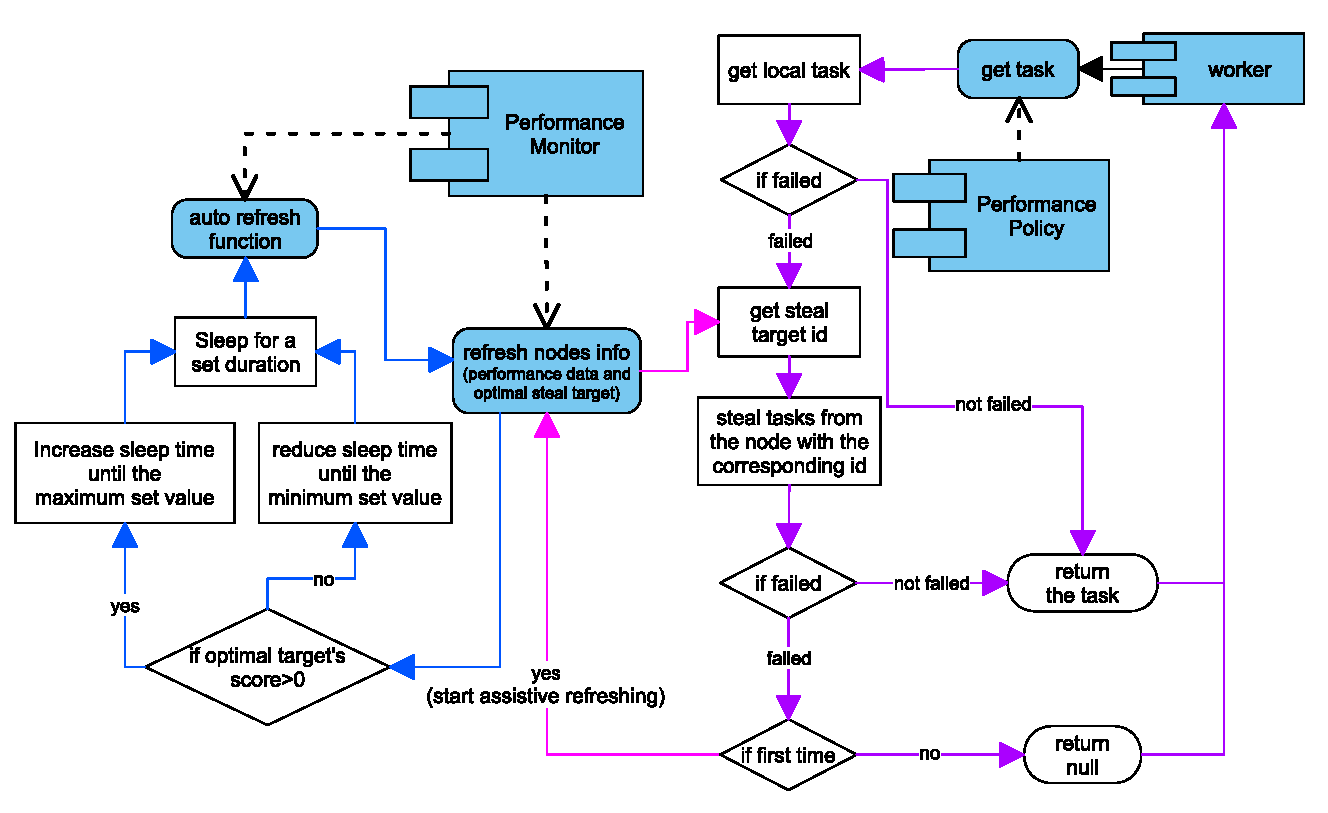
\includegraphics[width=0.98\textwidth]{images/refresh.pdf} % 插入图片,设置图片宽度为文本宽度的80%
    \caption{refresh data and provide tasks mechanism} % 提供图片的注解
    \label{fig:refresh_provide} % 为图片提供一个标签,以便在文档的其他地方引用
\end{figure}
\FloatBarrier

在图的左侧,是在Performance Monitor中部署的自动动态刷新任务,
它的本质上是一个循环,在每次刷新数据后都会根据刷新结果动态调整下一次刷新的时间,
如果刷新数据的结果不理想,
则说明当前很可能仍有worker处在饥饿的状态,
则会大幅缩短下一次刷新的时间;
但如果刷新数据的结果符合预期,
则说明workers很可能都会成功获取到任务进行执行,
所以会逐渐增加下一次刷新的时间,
避免频繁的刷新影响worker的计算性能.
而刷新数据的结果是否理想目前主要通过score进行判断,
目前的算法是如果score小于等于0则说明不理想,
因为根据\cref{eq:score}大概率是任务池任务数过少或者获取任务耗时过长导致的,
这种情况下,很可能会导致窃取的成本高于收益,
比如窃取时目标节点已无任务可窃取,
或者窃取的通讯延迟时间和本地执行时间相加不如远程节点自己执行完剩余任务的时间短等.
这里需要说明的是,虽然动态调整时间在实践中收益明显,
但是仍需要设置上下限,
因为如果不设置上限很可能导致由于落后的数据导致缓存了的错误窃取目标,
而如果不设置下限则会导致频繁的刷新影响了其它仍有任务执行的worker的性能或者影响系统底层的调度,
而如何界定这个上下限的值通过后续的多次实验,
发现在一定范围内既能达到对系统性能影响较低,又能保障数据的相对实时性,
而之前的通过加入了指数平滑等算法设计,
通过一定程度保留了历史数据的影响,
导致了数据即使有一定的延迟也能较为准确的反应各节点的综合情况.

而上述设计仍有不足之处与优化的空间,
所以还设计了如\cref{fig:refresh_provide}的右侧所示的一种通过Performance Policy进行辅助刷新的机制,
Performance Policy的本质是获取任务的一个策略,
它会优先获取本地的任务进行执行,
因为如果本地有任务的话会让worker更快地获取到任务并执行,
避免计算资源的浪费,
但是如果本地获取不到任务,
则会优先对Performance Monitor的最优窃取目标的id缓存进行查询,
通过获取的id对远程对应节点的任务池进行窃取,
这样大概率会窃取到有效的任务返回给worker进行执行,
从而尽可能避免worker的饥饿状态,
但是当各节点任务剩余数量都很少等情况下,
有小概率会无法窃取到任务,
这种在初期刚开始逐步生成任务,
或者在各节点都快执行完任务且很少有新任务加入时的情况下会出现的较多.
而自动刷新机制有可能此时在休眠状态无法及时调整刷新时间,
此时被woker调用的Performance Policy就会担任辅助刷新的作用,
主动去同步执行刷新数据的任务,
因为一方面不刷新数据则大概率这个worker还是会处于饥饿状态,
另一方面刷新数据时会占用这个worker的计算资源,而不会去影响其它worker,
但是如果获取到有效的窃取目标则会给自己和其它worker都带来收益,
当刷新数据完成后会再次尝试根据新的目标窃取一次任务,
如果还是失败则大概率说明当前各节点都很少有任务,
为了避免通讯等资源的占用,此时会返回空数据让这个worker进入休眠周期避免资源的占用.

而在实际实践中也发现两套机制互相配合能够很好地提升系统的性能.

%%%%%%%%%%%%%%%%%%%%%%%%%%%%%%%%%%%%%%%%%%%%%%%%%%%%%%%%%%%%%%%%%%%
\chapter{Evaluation}

\section{Search Applications}

我们对YewPar原有的两种搜索类型的代表性搜索应用和代表性样本上评估改进workstealing策略后的性能,
如下所示.

\begin{itemize}
    \item Enumeration:
          非平衡树搜索(UTS)根据给定的分支因子、深度和随机种子动态地构建合成的不规则树工作负载\cite{olivier2006uts}.
          数字半群(NS)计算具有特定属数的数字半群有多少\cite{fromentin2016exploring}.
          数字半群S是一个包含0且在加法下封闭的自然数的余集;
          S的属数是其补数的大小.
    \item Optimisation:
          最大团(MaxClique)找到给定图中的最大团,
          即最大的两两相邻顶点的集合。
          0/1背包问题确定将每个具有利润和重量的物品放入容器中的最佳组合,
          使得在给定的重量限制下利润最大化。旅行商问题(TSP)找到N个城市的最短循环之旅。
\end{itemize}

为了控制变量,
评估使用的应用程序maxclique-16和NS-hivert是YewPar的hpx1.8分支自带的应用程序,
并未对其进行改动,
其中MaxClique\cite{mccreesh2013multithreading}、
NS\cite{fromentin2016exploring}的基线实现使用了公开的先进算法.
这些顺序的C++实现是由领域专家提供的.
关于应用程序和实例的完整描述在\cite{archibald2018}中.


\section{Experimental Setup}
我们在多达20台机器上对程序运行情况进行了测量,
每台机器都配备了双8核的Intel Xeon E5-2640v2 2GHz CPU(无超线程),
64GB RAM,运行Ubuntu 22.04.2 LTS系统。
每台机器在测试前负载均在1\%之内,
我们为HPX(版本1.8)和原版的hpx1.8分支的YewPar一样预留了一个核心用于任务管理,
即在16个核心上我们使用15个工作线程。
需要注意的是,
由于修剪导致的非确定性、寻找替代有效解决方案和原版的YewPar的工作窃取方案具有较高的随机性,
并行搜索的性能分析是非常困难的,
这可能导致性能异常\ref{sec:performance_anomalies},
表现为超线性加速/减速.
为了控制这些因素,
我们对多种不同的节点数量下多次运行每个实验,
报告累计统计数据.

\section{空闲环境下加速效果评估}

为了准确评估基于Performance-Driven Workstealing Policy的YewPar与原版在空闲环境下的性能差异,
我们在各节点均处于空闲状态时,
对两种应用进行了独立的测试评估。
在这些测试中,运行的程序可以独占所有计算资源。










%%%%%%%%%%%%%%%%%%%%%%%%%%%%%%%%%%%%%%%%%%%%%%%%%%%%%%%%%%%%%%%%%%%
\chapter{Conclusion}\label{conclusion}

Main conclusions of your project. Here you should also include suggestions for future work.

\section{future work}


\appendix % first appendix
%%%%%%%%%%%%%%%%%%%%%%%%%%%%%%%%%%%%%%%%%%%%%%%%%%%%%%%%%%%%%%%%%%%
\chapter{First appendix}

\section{Section of first appendix}

%%%%%%%%%%%%%%%%%%%%%%%%%%%%%%%%%%%%%%%%%%%%%%%%%%%%%%%%%%%%%%%%%%%
\chapter{Second appendix}

%%%%%%%%%%%%%%%%%%%%%%%%%%%%%%%%%%%%%%%%%%%%%%%%%%%%%%%%%%%%%%%%%%%
% it is fine to change the bibliography style if you want
\bibliographystyle{plain}
\bibliography{mproj}
\end{document}
